\documentclass[]{article}
\usepackage[utf8]{inputenc}
\usepackage[margin=1.0in]{geometry}
\usepackage{amsmath, amsfonts}
\usepackage{tikz}
\usepackage[english]{babel}
\usepackage{amsthm}
\usepackage{mathtools}
\usepackage{enumitem}
\usepackage{graphicx}
\usepackage{fancyhdr}
\usepackage{subcaption}
\usepackage{unitsdef}
\usepackage{float}

\newtheorem{theorem}{Theorem}
\newtheorem{corollary}{Corollary}[theorem]
\renewcommand{\theenumi}{\Alph{enumi}}

\newcommand{\bd}{\textbf}
\newcommand{\del}{\nabla}
\newcommand{\by}{\times}
\newcommand{\R}{\mathbb R}
\newcommand{\C}{\mathbb C}
\newcommand{\M}{\mathcal M}
\newcommand{\Borel}{\mathcal B_{\mathbb R}}


\title{PHYS 506 Homework 1}
\date{Due 2/6}
\author{Kale Stahl}

\pagestyle{fancy}
\fancyhf{}
\makeatletter
\lhead{\@title}
\chead{\@date}
\rhead{\@author}
\makeatother

\begin{document}
	
	%Makes fancy title
	\makeatletter
	\begin{center}
		{\centering \Large \bd \@title}\\
		\vspace{.5cm}
		{\large \@author}
		\vspace{.25cm}
	\end{center}
	\makeatother
	
	\section*{Problem 1}
		Propagate uncertainty in each of the following. Explain what method you are using and why. Give both symbolic and numeric answers.
		\begin{enumerate}[label = \bd{(\alph*)}]
			\item $y = d\sin \theta$ for $d = (2.00\pm 0.05)$ m, $\theta = (15 \pm 1)\deg$.
			\item $P = (V-IR)I$ for $V = 5.0 \pm 0.2$ V, $I = 1.24 \pm 0.03$ A, $R = 0.13 \Omega \pm 5\%$
			\item $y = \sin \theta - \theta$ for $\theta = 0.000 \pm 0.087$ radians.
		\end{enumerate}
		\subsection*{Solution}
			\begin{enumerate}[label = \bd{(\alph*)}]
				\item This is a multiplication of 2 uncertain values, so we see
				\[
					\frac{\delta y}{y} = \sqrt{\left(\frac{\delta d}{d}\right)^2+\left(\frac{\delta (\sin \theta)}{\sin \theta}\right)^2}
				\]
				To calculate $\delta (\sin \theta)$ we must use the fact that this is a function of a single variable, so we have 
				\[
					\delta (\sin \theta) = \delta \theta \frac{\partial }{\partial \theta}(\sin \theta) = \delta \theta\cos \theta
				\]
				So then we have
				\begin{align*}
					\frac{\delta y}{y} &= \sqrt{\left(\frac{\delta d}{d}\right)^2+\left(\frac{\delta (\sin \theta)}{\sin \theta}\right)^2}\\
					 &= \sqrt{\left(\frac{\delta d}{d}\right)^2+\left(\frac{\delta \theta\cos \theta}{\sin \theta}\right)^2}\\
					\Aboxed{\delta y &= y\sqrt{\left(\frac{\delta d}{d}\right)^2+\left(\delta \theta\cot \theta\right)^2}}				\end{align*}
				So then numerically we have 
				\[
					y = (2.00 \meter)\sin (15 \deg) = 0.518 \meter
				\]
				\[
					\delta y =  (0.518 \meter)\sqrt{\left(\frac{0.05 \meter}{2.00 \meter}\right)^2+\left((1\deg \cdot 2\pi/360)
						\cot(15 \deg)\right)^2} = 0.0361 \meter 
				\]
				So our final value is 
				\[
					\boxed{y\pm \delta y = 0.518\pm 0.0361 \meter}
				\]
				\item This is simply a series of linear arithmetic operations, so we can simply add the proportional uncertainties in quadrature. We see
				\[
					\frac{\delta P}{P} = \sqrt{\left(\frac{\delta V}{V}\right)^2 + \left(\frac{\delta I}{I}\right)^2 + \left(\frac{\delta R}{R}\right)^2+ \left(\frac{\delta I}{I}\right)^2} =\sqrt{\left(\frac{\delta V}{V}\right)^2 + 2\left(\frac{\delta I}{I}\right)^2 + \left(\frac{\delta R}{R}\right)^2}
				\]
				So then numerically we have 
				\[
					P = (5.0 - (1.24)(0.13))(1.24)= \boxed{6.00} 
				\]
				\[
					\delta P = (6.00)\sqrt{\left(\frac{0.2}{5.0}\right)^2 + 2\left(\frac{0.03}{1.24}\right)^2 + \left(.05\right)^2} = \boxed{.4107}
				\]
				\item We see that the graph is given by
				\begin{figure}
					\centering
					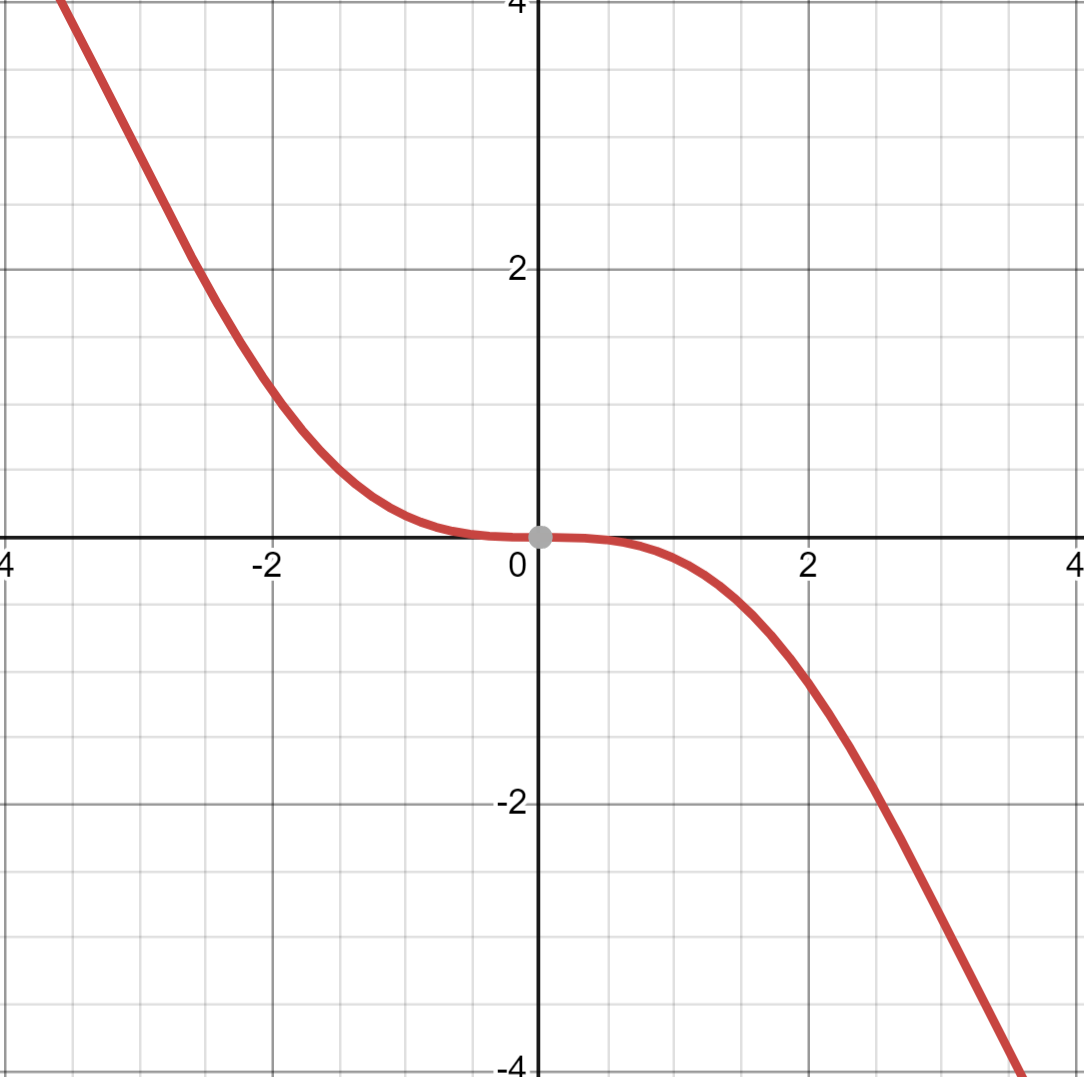
\includegraphics[width = .5\textwidth]{C:/Users/kales/OneDrive/Desktop/PHYS 506 - Advanced Lab/Homework/HW 1 1c.png}
				\end{figure}
				This is approximately linear in a neighborhood of zero, so we can simply use the first order Taylor approximation and use the fact that $\sin x\approx x$ about zero. So then the uncertainty in $y$ is given by the same uncertainty in $x$. The use of any other method should result in the uncertainty being zero, which cannot be reasonable.
			\end{enumerate}
	\section*{Problem 2}
		n experiment measures the rate of a certain type of cosmic ray over 16 years, exactly
		5844 days. They divide the data by “season” into 4 equal-sized data sets, each 1461
		days long. They observe 771, 762, 686, and 802 events in the spring, summer, fall,
		and winter data sets respectively. The expected “background” of false events in each
		data set is $\mu_B = 51.4$. The number of events observed by the experiment in season $i$ is
		expected to be a Poisson random variable with mean $\mu_i = \mu_{Ci} + \mu_B$, where $\mu_{Ci}$ is the
		actual mean rate expected number of cosmic rays in that season. Find:
		\begin{enumerate}[label = \bd{(\alph*)}]
			\item Best estimate and standard (1-sigma) uncertainty for $\mu_{Ci}$ for each season.
			\item Best estimate for overall mean rate number $\mu_C$ of the cosmic rays averaged over all seasons.
			\item Deviation $\Delta \mu_{Ci}$ of the mean rate count in each 16-season bin from the yearly
			mean, with uncertainty.
		\end{enumerate}
		\subsection*{Solution}
			\begin{enumerate}[label = \bd{(\alph*)}]
				\item Since these counts are relatively large, the uncertainty in the Poisson counts can simply be given by the square root of the counts. So taking into account the fact that $\mu_i = \mu_{Ci} + \mu_B$, we see the following:
				\begin{itemize}
					\item\bd{Spring:} $\mu_{C1} = 771- 51.4 = $, so then $\Delta \mu_{C1} =719.6 \sqrt{\mu_{C1}} = 26.8$
					\item \bd{Summer:} $\mu_{C2} = 762- 51.4 = $, so then $\Delta \mu_{C2} = 710.4 \sqrt{\mu_{C2}} = 26.66$
					\item \bd{Fall:} $\mu_{C3} = 686- 51.4 = $, so then $\Delta \mu_{C3} = 634.6 \sqrt{\mu_{C3}} = 25.19$
					\item \bd{Winter:} $\mu_{C4} = 802- 51.4 = $, so then $\Delta \mu_{C4} =750.6 \sqrt{\mu_{C4}} = 27.4$
				\end{itemize}
				\item For to find the value, we simply take the arithmetic mean over the four seasons. We see
				\[
					\mu_C = \frac{771+762+686+802}{4}=755
				\]
				and the uncertainty in this mean is given by
				\[
					\sigma_{\mu_C} = \sqrt{\frac{(771- 755)^2+(762-755)^2+(686-755)^2+(802- 755)^2}{3}} = 50.2
				\]
				So then we estimate our mean count to be $\mu_C = 755 \pm 50.2$ counts.
				\item 
				There is only one measurement for each season, so our deviation is merely the difference of the two values and the uncertainty would be given by adding the uncertainties in quadrature.
			\end{enumerate}
	\section*{Problem 3}
		The formula for double weighing on a balance is $W =
		p + \frac{r_1 - r_2}{2s}$
		, in which $p$ is the sum of the weights used, $r1$ and $r2$ are the pointer
		readings when object is on left and right pans, respectively, and s is the sensibility of
		the balance [in pointer units per weight unit]. For ten weighings of the same object,
		the values of $r_1 -r_2$ were as follows: 0.96, 0.93, 1.08, 0.95, 0.99, 1.12, 1.02, 1.05, 0.92,
		1.10. The factor $\frac{1}{2s}$ for the load used was 0.0002753 [grams per pointer unit]. Find the probable error of one weighing, and of the mean of the ten weighings. (Does $p$ need to
		be given for this purpose?)
		\subsection*{Solution}
			Since these are random samples, we will assume that the distribution is approximately Gaussian. So then the probable uncertainty of a single measurement is given as the standard deviation. We have symbolically
			\[
				\sigma_W = \sqrt{\frac{1}{9}\sum^{10}_{i=1}\left(\left(p + \frac{1}{2s}x_i\right) - \mu_W\right)^2}
			\]
			Where $\mu$ is given as the mean or 
			\[
				\mu_W = \frac{1}{10}\sum_{i=1}^{10}\left(p + \frac{1}{2s}x_i\right) = p + \frac{1}{20s}\sum_{i}x_i
			\]
			So then
			\[
				\sigma_W = \sqrt{\frac{1}{9}\sum^{10}_{i=1}\left(\left(p + \frac{1}{2s}x_i\right) - \left(p + \frac{1}{20s}x_i\right)\right)^2} = \sqrt{\frac{1}{9}\sum^{10}_{i=1}\left( \frac{9}{20s}x_i\right)^2} 
			\]
			So then numerically we have 
			\begin{align*}
				\sigma_W &= \frac{1}{2s}\frac{3}{10}\sqrt{\sum^{10}_{i=1} x_i^2}\\
				&= \frac{3}{10}(.002753)\sqrt{0.96^2+ 0.93^2+1.08^2+0.95^2+0.99^2+1.12^2+1.02^2+1.05^2+0.92^2+1.10^2} = 0.00265
			\end{align*}
			And the expected error of the average will be this number divided by the square root of the number of measurements, so we have 
			\[\sigma_{\mu_W} = \frac{\sigma_W}{\sqrt{10}} = 0.00008377\]
			We do not need $p$ for either of these calculations as it always cancels out.
	\section*{Problem 4}
		Problem 4.28 from [Taylor]
		\subsection*{Solution}
		\begin{enumerate}[label = \bd{(\alph*)}]
			\item For our values, we see
			\begin{figure}[h]
				\centering
				\begin{tabular}{|c|c|c|c|c|c|}
					\hline
					&1&2&3&4&5\\
					\hline
					$l$&51.2&59.7&68.2&79.7&88.3\\
					$T$&1.448&1.566&1.669&1.804&1.896\\
					$g$&964.03&961.06&966.57&966.82&969.71\\
					\hline
				\end{tabular}
			\end{figure}
			The mean of the 5 measurements of $g$ is $\mu_g = 965.638$. So then the standard deviation is given by
			\[
				\sigma = \sqrt{\frac{(965.638-964.03 )^2+ (965.638- 961.06)^2+(965.638-966.57 )^2+(965.638- 966.82)^2+(965.638-969.71)^2}{4}} = 3.26
			\]
			So then the SDOM is given by
			\[
				\sigma_\mu = \frac{\sigma}{\sqrt{5}} = \boxed{1.456}
			\]
			\item If the accepted value is 979.6, then the difference is $14.038$ which is indeed almost 10 times more than our error estimate.
			\item For the error value to just include the accepted value, we first note that the function used has only one systematic uncertainty, so the uncertainty in $l$ will be the uncertainty in $g$. So then our absolute uncertainty must be $14.038$ and our fractional uncertainty must be $14.038/965.638 = .0145$ which is indeed around 1.5\%.
			\item For our new values, we see
			\begin{figure}[h]
				\centering
				\begin{tabular}{|c|c|c|c|c|c|}
					\hline
					&1&2&3&4&5\\
					\hline
					$l$&53.2&61.7&70.2&71.7&90.3\\
					$T$&1.448&1.566&1.669&1.804&1.896\\
					$g$&1001.69&993.256&994.91&869.77&991.69\\
					\hline
				\end{tabular}
			\end{figure}
			The mean of the 5 measurements of $g$ is $\mu_g = 970.26$. So then the standard deviation is given by
			\[
			\sigma = \sqrt{\frac{(970.26-964.03 )^2+ (970.26- 961.06)^2+(970.26-966.57 )^2+(970.26- 966.82)^2+(970.26-969.71)^2}{4}} = 2.64
			\]
			So then the SDOM is given by
			\[
			\sigma_\mu = \frac{\sigma}{\sqrt{5}} = \boxed{1.18}
			\]
		\end{enumerate}
		
\end{document}
?